\documentclass[main.tex,fontsize=8pt,paper=a4,paper=portrait,DIV=calc,]{scrartcl}
% Document
\usepackage[T1]{fontenc}
\usepackage[utf8]{inputenc}
\usepackage[dvipsnames]{xcolor}
\usepackage[nswissgerman,english]{babel} 
\usepackage{hyperref}
\renewcommand{\familydefault}{\sfdefault}

% Format
\usepackage[top=5mm,bottom=1mm,left=5mm,right=5mm]{geometry}
%\setlength{\headheight}{\baselineskip}
%\setlength{\headsep}{0mm}

%\usepackage{scrlayer-scrpage}
%\clearpairofpagestyles
%\chead{{\bfseries\TITLE, \AUTHOR, \pagename~\thepage}}

%\addtokomafont{pagehead}{\upshape}

\usepackage{multicol}
\setlength{\columnsep}{2mm}
\setlength{\columnseprule}{0.1pt}

% Math
\usepackage{amsmath}
\usepackage{amssymb}
\usepackage{amsfonts}

% Code
\usepackage{fancyvrb, etoolbox, listings, xcolor}
%\usemintedstyle{bw}

%\newminted[shell]{bash}{
%fontsize=\footnotesize,
%fontfamily=tt,
%breaklines=true,
%frame=single,
%framerule=0.1pt,
%framesep=2mm,
%tabsize=2
%}
%\newminted{css}{
%breaklines=true,
%tabsize=4,
%autogobble=true,
%escapeinside=||,
%stripall=true,
%stripnl=true,
%}

    \definecolor{lightgray}{rgb}{0.95, 0.95, 0.95}
    \definecolor{darkgray}{rgb}{0.4, 0.4, 0.4}
    \definecolor{purple}{rgb}{0.65, 0.12, 0.82}
    \definecolor{ocherCode}{rgb}{1, 0.5, 0} % #FF7F00 -> rgb(239, 169, 0)
    \definecolor{blueCode}{rgb}{0, 0, 0.93} % #0000EE -> rgb(0, 0, 238)
    \definecolor{greenCode}{rgb}{0, 0.6, 0} % #009900 -> rgb(0, 153, 0)
    \definecolor{teal}{rgb}{0.0, 0.5, 0.5}

\lstdefinestyle{code}{
    identifierstyle=\color{black},
    keywordstyle=\color{blue}\bfseries\small,
    ndkeywordstyle=\color{greenCode}\bfseries\small,
    stringstyle=\color{ocherCode}\ttfamily\small,
    commentstyle=\color{teal}\ttfamily\textit\small,
    basicstyle=\ttfamily\small,
    breakatwhitespace=false,         
    breaklines=true,                 
    captionpos=b,                    
    keepspaces=true,                 
    showspaces=false,                
    showstringspaces=false,
    showtabs=false,                  
    tabsize=2,
    belowskip=-5pt
}



% Images
\usepackage{graphicx}
\newcommand{\pic}{\includegraphics[scale=0.3]}
\graphicspath{{Screenshots/}{../Screenshots}}
\makeatletter
\def\pictext#1#2{%
    \@ifnextchar[{%
    \pictext@iiiii{#1}{#2}%
    }{%
      \pictext@iiiii{#1}{#2}[0.5,0.4,0.3]% Default is 5
    }%
}
\def\pictext@iiiii#1#2[#3,#4,#5]{\begin{minipage}{#3\textwidth}\includegraphics[scale=#4]{#1}\end{minipage}\begin{minipage}{#5\textwidth}#2\end{minipage}}
\def\minipg#1#2{%
    \@ifnextchar[{%
    \minipg@iiii{#1}{#2}%
    }{%
      \minipg@iiii{#1}{#2}[0.3,0.6]% Default is 5
    }%
}
\def\minipg@iiii#1#2[#3,#4]{\vspace{0.8mm}\begin{minipage}{#3\textwidth}#1\end{minipage}\begin{minipage}{#4\textwidth}#2\end{minipage}{\vspace{0.8mm}}}
\makeatother

%\newenvironment{minty}[2]% environment name
%{% begin code
%  \begin{minipage}{#1}
%  \begin{minted}{#2}
%}%
%{% end code
%  \end{minted}
%  \end{minipage}
%  \end{minty}\ignorespacesafterend
%} 

% Smaller Lists
\usepackage{enumitem}
\setlist[itemize,enumerate]{leftmargin=3mm, labelindent=0mm, labelwidth=1mm, labelsep=1mm, nosep}
\setlist[description]{leftmargin=0mm, nosep}
\setlength{\parindent}{0cm}

% Smaller Titles
\usepackage[explicit]{titlesec}

%% Color Boxes
\newcommand{\sectioncolor}[1]{\colorbox{black!60}{\parbox{0.989\linewidth}{\color{white}#1}}}
\newcommand{\subsectioncolor}[1]{\colorbox{black!50}{\parbox{0.989\linewidth}{\color{white}#1}}}
\newcommand{\subsubsectioncolor}[1]{\colorbox{black!40}{\parbox{0.989\linewidth}{\color{white}#1}}}
\newcommand{\paragraphcolor}[1]{\colorbox{black!30}{\parbox{0.989\linewidth}{\color{white}#1}}}
\newcommand{\subparagraphcolor}[1]{\colorbox{black!20}{\parbox{0.989\linewidth}{\color{white}#1}}}

%% Title Format
\titleformat{\section}{\vspace{0.5mm}\bfseries}{}{0mm}{\sectioncolor{\thesection~#1}}[{\vspace{0.5mm}}]
\titleformat{\subsection}{\vspace{0.5mm}\bfseries}{}{0mm}{\subsectioncolor{\thesubsection~#1}}[{\vspace{0.5mm}}]
\titleformat{\subsubsection}{\vspace{0.5mm}\bfseries}{}{0mm}{\subsubsectioncolor{\thesubsubsection~#1}}[{\vspace{0.5mm}}]
\titleformat{\paragraph}{\vspace{0.5mm}\bfseries}{}{0mm}{\paragraphcolor{\theparagraph~#1}}[{\vspace{0.5mm}}]
\titleformat{\subparagraph}{\vspace{0.5mm}\bfseries}{}{0mm}{\subparagraphcolor{\thesubparagraph~#1}}[{\vspace{0.5mm}}]

%% Title Spacing
\titlespacing{\section}{0mm}{0mm}{0mm}
\titlespacing{\subsection}{0mm}{0mm}{0mm}
\titlespacing{\subsubsection}{0mm}{0mm}{0mm}
\titlespacing{\paragraph}{0mm}{0mm}{0mm}
\titlespacing{\subparagraph}{0mm}{0mm}{0mm}

%% format cells
\usepackage[document]{ragged2e}
\usepackage{array, makecell}
\renewcommand{\arraystretch}{2}
\newcommand{\mc}{\makecell[{{m{1\linewidth}}}]}



\begin{document}
\tableofcontents

\lstset{
    language=Python,
    style=code,
}

\newcommand{\TITLE}{AI Applications}
\newcommand{\AUTHOR}{Fabio Lenherr}
\setcounter{tocdepth}{1}

\section{CNN Convolutional Neural Networks}

\subsection{Keras}
A python library that wraps tensorflow for classification.\newline
We will use this in this module to classify images like so:\newline
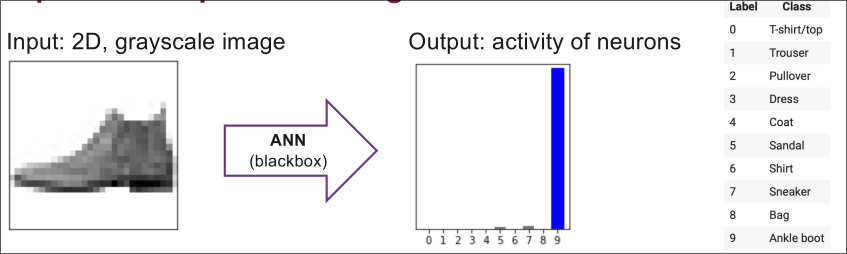
\includegraphics[scale=0.4]{2023_02_20_12_32_47.png}

\subsection{Flattening}
When we convert an image into a long vector, we lose information in the human sense, or rather make it hidden.\newline
todo, explain what is hidden and why


\section{Convolution}
\subsection{Firing of neurons}
Neurons are clearly connected to something very specific, this would then also be reflected in the artificial neural network. In other words, neuron 1 handles horizontal lines, another a line with a slight angle and so-on.\newline
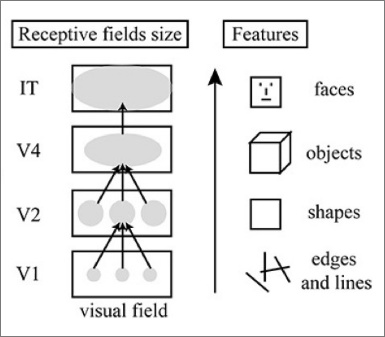
\includegraphics[scale=0.4]{2023_02_20_02_19_00.png}

\subsection{mathematical model of a feature detector}
\begin{itemize}
\item \textcolor{purple}{Two Inputs}\newline
  \begin{itemize}
  \item \textcolor{orange}{a picture}\newline
    Note that rgb would give you 3 channels red, green and blue
  \item \textcolor{orange}{A filter(kernel)}\newline
  \begin{itemize}
  \item  an m by n matrix in the simplest case (1 channel, grayscale).
  \item an m by n x 3 "stack of matrices" in the case of a 3 channel input (e.g. an RGB image)
  \item an m by n x d "stack of matrices". The depth of the kernel must equal the number of input channels.
  \end{itemize} 
\end{itemize} 
\item \textcolor{purple}{One Output}\newline
  A feature map (where is the thing that we wanted to search / determine by)\newline
  One convolution produces one feature map. Even if the input and the filter have multiple channels, the output of the convolution has one channel.
\item \textcolor{purple}{The Operation: Convolution}\newline
  We convolve the input image with the convolutional kernel
\end{itemize} 

\subsection{Example of convolution}
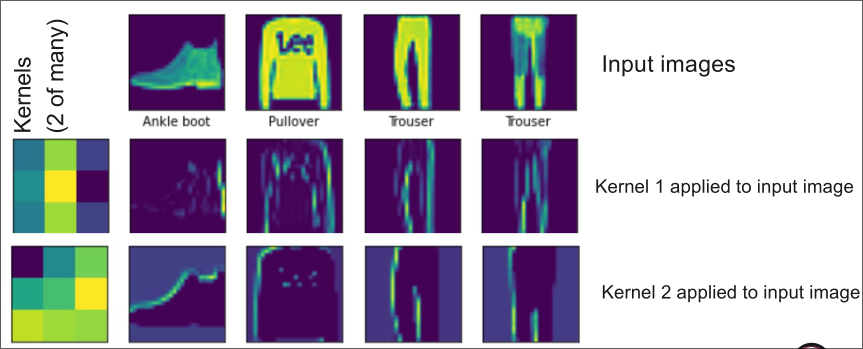
\includegraphics[scale=0.4]{2023_02_20_02_23_12.png}\newline
As you can see here, a filter will be used to detect something specific, like a pattern.\newline
\textcolor{purple}{This means that you will be combining multiple different filters in order to properly figure out what picture the underlying image is composed of.}\newline
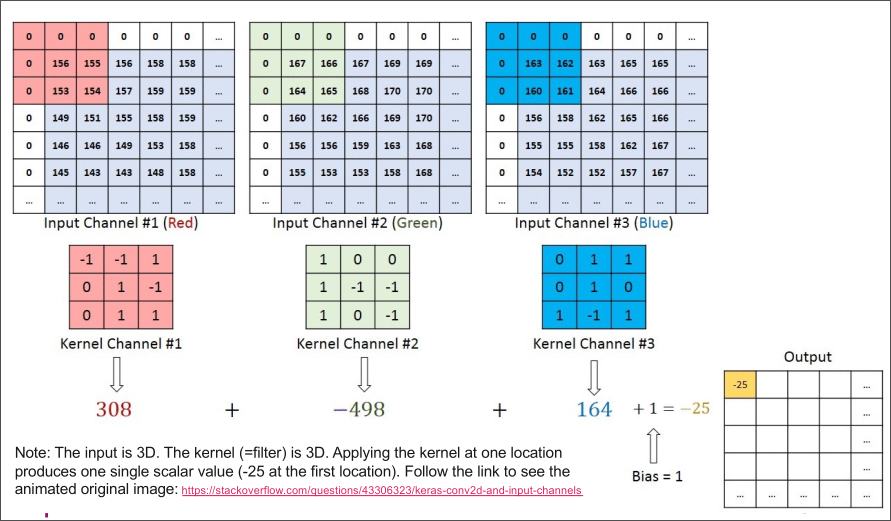
\includegraphics[scale=0.4]{2023_02_20_02_23_46.png}\newline
\textcolor{purple}{Explanation for the first calculation: 0 * -1 + 0 * -1 + 0 * 1 + 0 * 0 + 156 * 1 + 155 * -1 + 0 * 0 + 153 * 1 + 154 * 1 = 308}\newline
multiply each number in the top red square with the number in the same position in the bottom square.
We then proceed to do this for all channels (complexity of input, 3 for rgb), which \emph{will then be combined to 1 single output value}.\newline
This output value will then also be combined with a \emph{bias}.\newline
\textcolor{purple}{The entire reason we do this, is so that we can have an easier time calculating the images with a pc.}

\subsection{Reasons for convolution}
\begin{itemize}
\item \textcolor{purple}{Features can be detected independent of location -> filters will always find what they are supposed/created to find}
\item \textcolor{purple}{This calculation is done in parallel, which is very fast for gpus when doing matrix calculations! -> Hence the use of tensorflow with cuda!}
\item \textcolor{purple}{Shared weights mean using the same \emph{kernel values}, this reduces the use of a singular value for each neuron. -> more processing etc}
\end{itemize} 

\subsection{Stride}
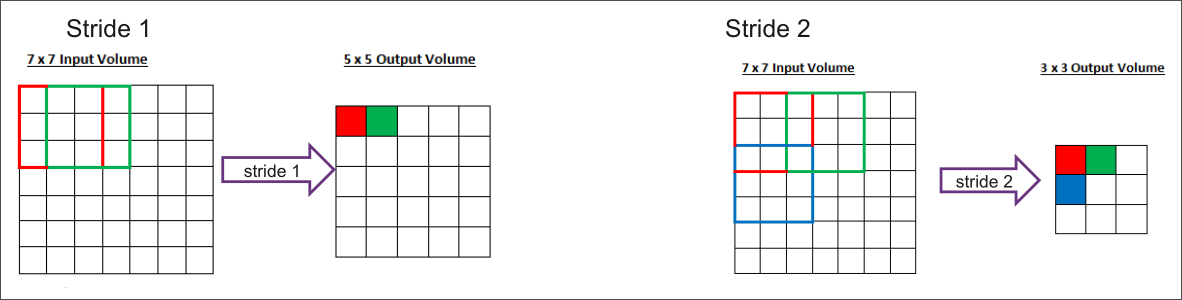
\includegraphics[scale=0.4]{2023_02_20_02_44_29.png}\newline
\textcolor{purple}{Stride is simply the offset by which we move towards the right and the bottom when we move to the next calculation.}\newline
The default value here is 1, which means Stride 1.

\subsection{Padding}
\minipg{
Padding is simply the edge of the matrix that has been predefined.\newline
A same padding is made entirely of 0's!\newline
\textcolor{purple}{Note, with padding, we can effectively go over the bounds of the matrix!}
}{
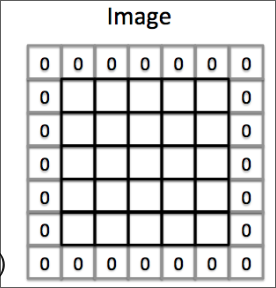
\includegraphics[scale=0.4]{2023_02_20_02_47_01.png}
}[0.45,0.4]

\subsection{Max Pooling}
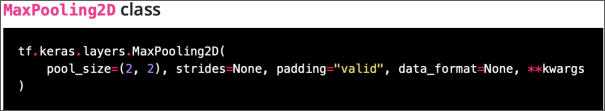
\includegraphics[scale=0.4]{2023_02_20_02_46_05.png}\newline
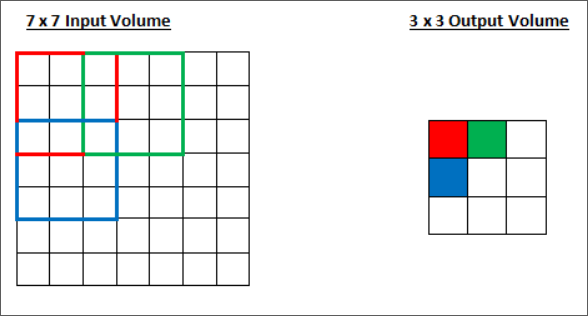
\includegraphics[scale=0.4]{2023_02_20_02_48_45.png}\newline
Max pooling simplyfies the image by taking the maximum value in each sector.\newline
For example in the first red square, the highest value will be placed in the right red square.\newline
Similar to before, we then iterate with the stride as the length to iterate and do this again and again until we are done.

\subsection{Example with Keras}
\begin{lstlisting}
model = Sequential([
  layers.Rescaling(1./255, input_shape=(img_height, img_width, 3)),
  layers.Conv2D(16, 3, padding='same', activation='relu'),
  layers.MaxPooling2D(),
  layers.Conv2D(32, 3, padding='same', activation='relu'),
  layers.MaxPooling2D(),
  layers.Conv2D(64, 3, padding='same', activation='relu'),
  layers.MaxPooling2D(),
  layers.Flatten(),
  layers.Dense(128, activation='relu'),
  layers.Dense(num_classes)
])
\end{lstlisting}
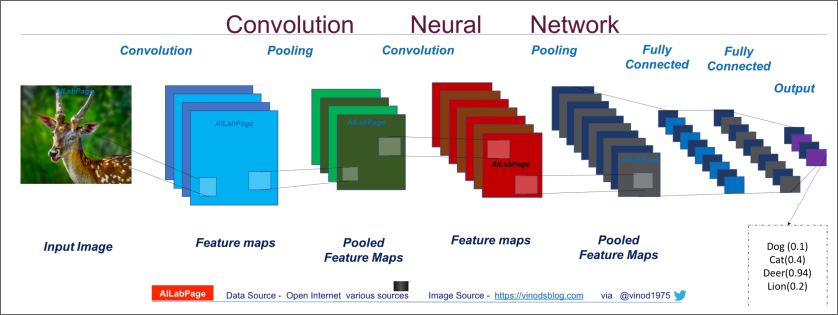
\includegraphics[scale=0.4]{2023_02_27_01_28_25.png}

\subsection{Softmax}
\textcolor{purple}{Softmax is used to get the probabilities of each classification.}
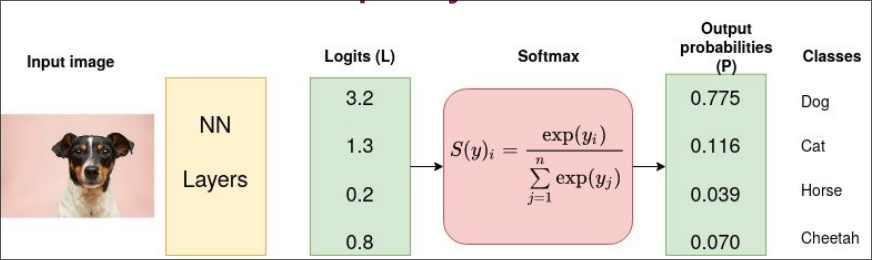
\includegraphics[scale=0.4]{2023_02_27_05_50_28.png}

\subsection{Drop Out}
\minipg{
\textcolor{purple}{This is similar but not quite the same as ensemble method learning.\newline
It is used to get models that are more robust than otherwise.}\newline
\textcolor{teal}{This entire ordeal is done during training, not during inference!}
}{
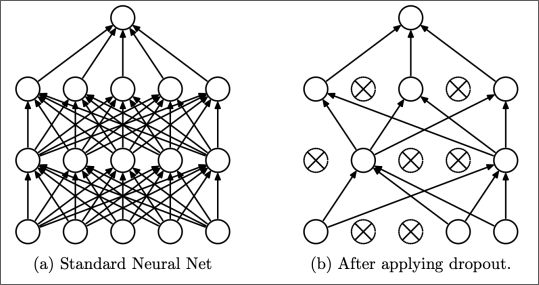
\includegraphics[scale=0.4]{2023_02_27_05_54_10.png}
}[0.45,0.45]

\subsection{Why?}
The entire filter is essentially just a shape, packed into a matrix.\newline
If you for example have a filter of a 2x2 matrix and you only fill the bottom left and top right square with one and the others with 0, then you will detect whether or not the shape in question has a diagonal line inside of it.\newline
Note that with the others being 0, you will \emph{ignore} the rest of the shape around it. This means you will detect ALL diagonal lines, \emph{even if they are within another shape.}.\newline
\textcolor{purple}{Should you want to only detect diagonal lines that have no other color around it, then you need to make the other values in the filter matrix as negative, indicating that you only want the diagonal lines that are isolated.}\newline
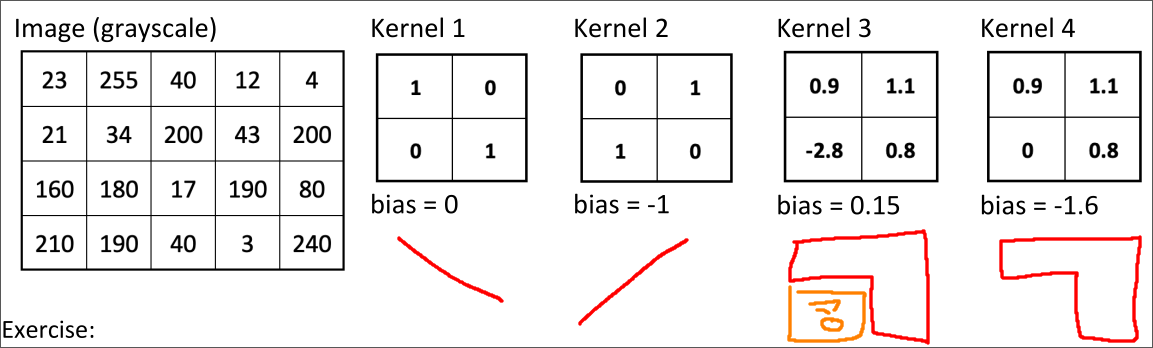
\includegraphics[scale=0.4]{2023_02_21_09_51_55.png}

\subsection{Tensor}
A tensor is just a multidimensional array. The structure is as follows:\newline
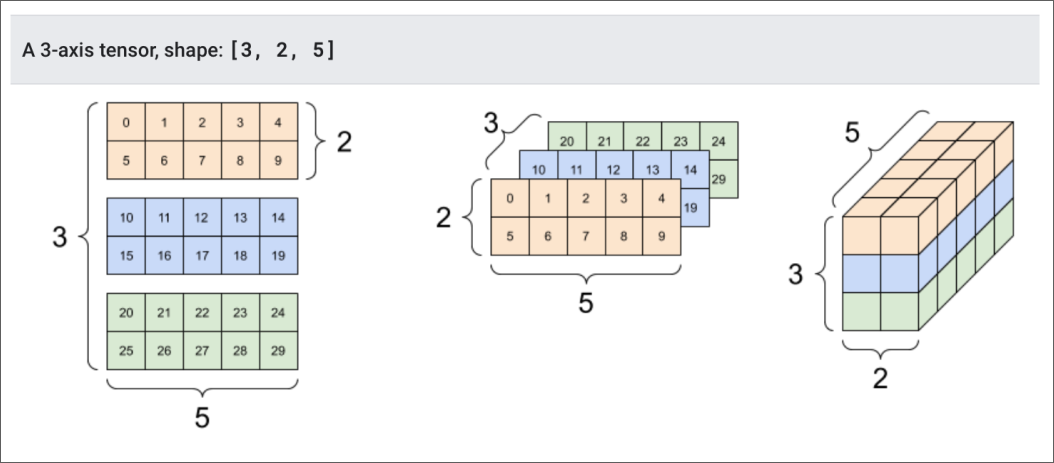
\includegraphics[scale=0.4]{2023_02_21_09_56_23.png}\newline
In other words: \textcolor{purple}{\emph{amount of sub-arrays, width of sub-array, length of sub-array}}\newline
\textcolor{teal}{Tensors are immutable, meaning you can only create new ones, you can't update them!}\newline
Terms:
\begin{itemize}
  \item \textcolor{orange}{Rank} \newline
    The amount of parameters, in the example we had rank3, but what if the sub-arrays had a height as well? -> rank 4!
\item \textcolor{orange}{Axis or Dimension}\newline
  a particular dimension of a tensor, remember 3 dimensions = rank3\newline
  A rank-4 tensor, shape: [3, 2, 4, 5]
\item \textcolor{orange}{Shape}\newline
  The length (number of elements) of each of the axes of a tensor.
\item \textcolor{orange}{Size}\newline
  The total number of items in the tensor, the product of the shape vector's elements.
\item \textcolor{orange}{Indexing}\newline
  simply the indexing of the array like in python.
  \begin{lstlisting}
  rank_1_tensor = tf.constant([0, 1, 1, 2, 3, 5, 8, 13, 21, 34])
  print(rank_1_tensor.numpy())
  print("First:", rank_1_tensor[0].numpy())
  print("Second:", rank_1_tensor[1].numpy())
  print("Last:", rank_1_tensor[-1].numpy())
  # First: 0
  # Second: 1
  # Last: 34
  \end{lstlisting}
\item \textcolor{orange}{Reshaping}\newline
  reshapes a vector by a given list. -> shape is a list!\newline
  Remember that the order and amount of axis need to match! Otherwise you get trash!
  \begin{lstlisting}
  # Shape returns a `TensorShape` object that shows the size along each axis
  x = tf.constant([[1], [2], [3]])
  print(x.shape)
  # You can reshape a tensor to a new shape.
  # Note that you're passing in a list
  reshaped = tf.reshape(x, [1, 3])
  print(x.shape)
  print(reshaped.shape)
  # (3, 1)
  # (1, 3)
  \end{lstlisting}
\item \textcolor{orange}{Broadcasting}\newline
  When tensors aren't the same size, you can essentially default extend them, in this case the last value will be taken.
  \begin{lstlisting}
  x = tf.constant([1, 2, 3])
  y = tf.constant(2)
  z = tf.constant([2, 2, 2])
  # All of these are the same computation
  print(tf.multiply(x, 2))
  print(x * y)
  print(x * z)
  # tf.Tensor([2 4 6], shape=(3,), dtype=int32)
  # tf.Tensor([2 4 6], shape=(3,), dtype=int32)
  # tf.Tensor([2 4 6], shape=(3,), dtype=int32)
  \end{lstlisting}
\end{itemize} 
\href{https://www.tensorflow.org/guide/tensor}{code tutorial}

\subsection{An example for image classification}
\begin{lstlisting}
# import necessary modules
import tensorflow as tf

from tensorflow.keras import datasets, layers, models
import matplotlib.pyplot as plt
(train_images, train_labels), (test_images, test_labels) = datasets.cifar10.load_data()

# Normalize pixel values to be between 0 and 1
train_images, test_images = train_images / 255.0, test_images / 255.0
class_names = ['airplane', 'automobile', 'bird', 'cat', 'deer',
               'dog', 'frog', 'horse', 'ship', 'truck']

# show pictures
plt.figure(figsize=(10,10))
for i in range(25):
    plt.subplot(5,5,i+1)
    plt.xticks([])
    plt.yticks([])
    plt.grid(False)
    plt.imshow(train_images[i])
    # The CIFAR labels happen to be arrays, 
    # which is why you need the extra index
    plt.xlabel(class_names[train_labels[i][0]])
plt.show()

# create convolutional base
model = models.Sequential()
model.add(layers.Conv2D(32, (3, 3), activation='relu', input_shape=(32, 32, 3)))
model.add(layers.MaxPooling2D((2, 2)))
model.add(layers.Conv2D(64, (3, 3), activation='relu'))
model.add(layers.MaxPooling2D((2, 2)))
model.add(layers.Conv2D(64, (3, 3), activation='relu'))

# Add dense layers on top 
model.add(layers.Flatten())
model.add(layers.Dense(64, activation='relu'))
model.add(layers.Dense(10))

# Compile and train the model
model.compile(optimizer='adam',
              loss=tf.keras.losses.SparseCategoricalCrossentropy(from_logits=True),
              metrics=['accuracy'])

# Evaluate the model
history = model.fit(train_images, train_labels, epochs=10, 
                    validation_data=(test_images, test_labels))
plt.plot(history.history['accuracy'], label='accuracy')
plt.plot(history.history['val_accuracy'], label = 'val_accuracy')
plt.xlabel('Epoch')
plt.ylabel('Accuracy')
plt.ylim([0.5, 1])
plt.legend(loc='lower right')
test_loss, test_acc = model.evaluate(test_images,  test_labels, verbose=2)

# print the accuracy at the end
print(test_acc)

\end{lstlisting}
\href{https://www.tensorflow.org/tutorials/images/cnn}{full tutorial}



\section{Encoder and Decoder}
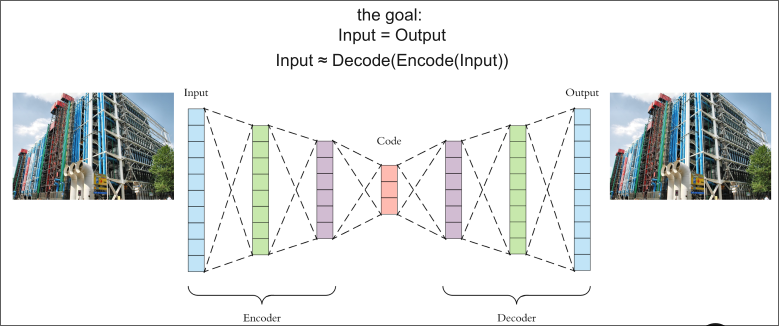
\includegraphics[scale=0.4]{2023_03_06_01_44_16.png}\newline
\textcolor{purple}{The idea here is that we can compress the data from the "noisy" picture into it's base shapes. \newline
While this means we will lose the detail, we will also lose the "noise", that came along with the picture.}\newline
\textcolor{orange}{Base ideas:}
\begin{itemize}
\item \textcolor{black}{Bottleneck layer -> force the image into smaller layers}
\item \textcolor{black}{code in the middle is \emph{a feature vector}}
\item \textcolor{black}{Base idea: if we know the structure, we do not need to know every pixel!}
\item Unsupervised learning, there are no labels!
\item transfer learning: reuse part of the network for other tasks
\end{itemize} 
\href{https://www.tensorflow.org/tutorials/generative/autoencoder}{Tutorial for Encoder}

\subsubsection{Audio transformation}
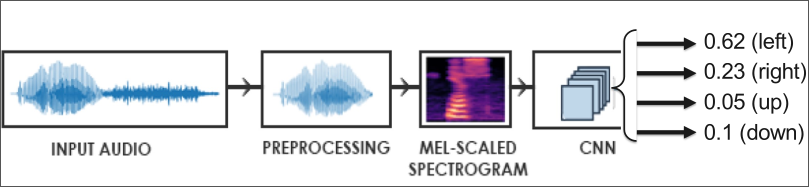
\includegraphics[scale=0.4]{2023_03_06_02_33_17.png}\newline
\textcolor{purple}{The idea here is that you take small portions of audio (11ms or something similar), then you turn the frequency table. This gives you the "modified" output on the right.}

\section{RNN}

\subsection{Sequential Data}
\textcolor{teal}{This is the 1 input 1 output criteria, basically the one thing haskell is actually quite good at!}\newline
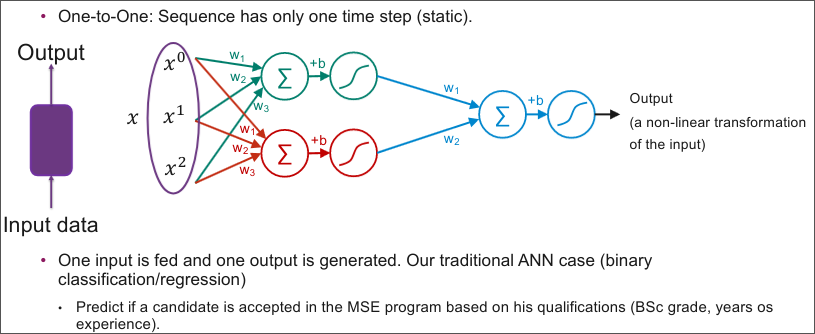
\includegraphics[scale=0.4]{2023_03_20_01_46_19.png}\newline
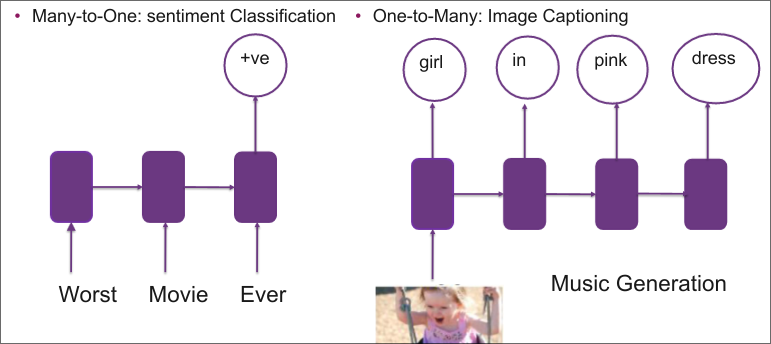
\includegraphics[scale=0.4]{2023_03_20_01_44_14.png}
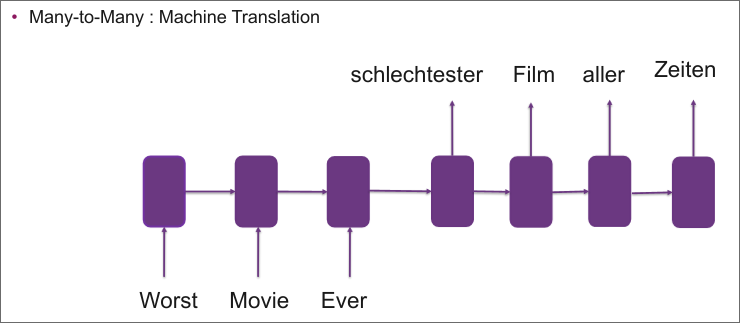
\includegraphics[scale=0.4]{2023_03_20_01_45_11.png}\newline
\textcolor{teal}{These are all fine, but the limitation is that we do not have a memory. So the usefulness is limited at best.}

\subsection{Dealing with memory}
When you need to remember about previous states, then you can't use ANN or CNN.\newline
\textcolor{teal}{For regular ANNs the problem is that they add things together and forget about the initial state.\newline
Take this FFNN for example:}\newline
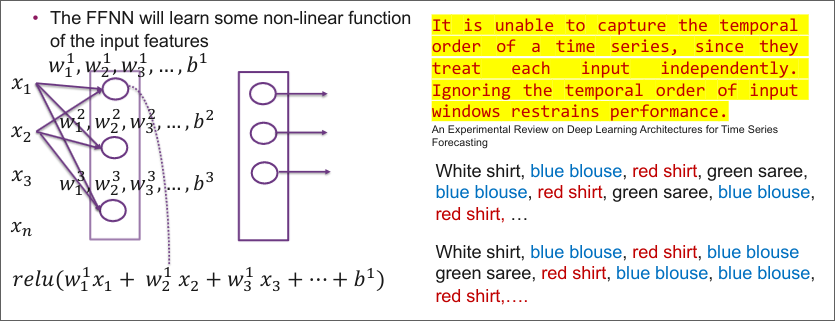
\includegraphics[scale=0.4]{2023_03_20_02_08_30.png}\newline
The problem here is that the FFNN adds together the inputs, meaning that you will not remember what the inputs were at the start.\newline
So how about CNN?\newline
\textcolor{teal}{For CNN the problem is that you only see whether or not somehting was/is there with a clear information loss.\newline
This means you can't remember the exact input, you only know, input class x was there!} 

\subsection{The Solution}
\subsubsection{How do we handle the time component?}
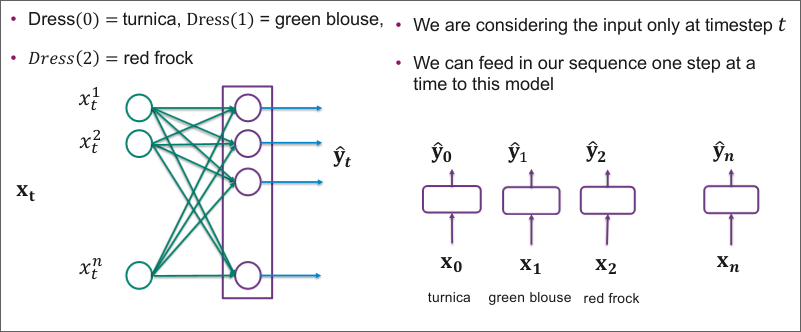
\includegraphics[scale=0.4]{2023_03_20_02_10_55.png}
\subsubsection{Adding Connections}
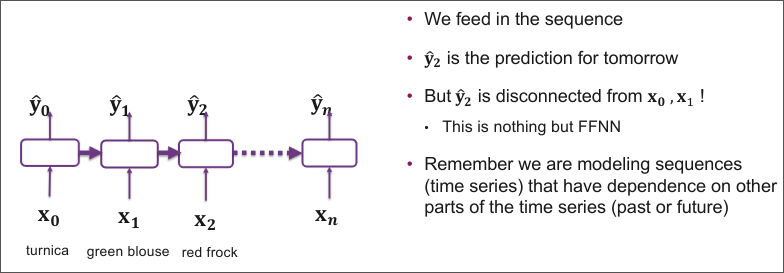
\includegraphics[scale=0.4]{2023_03_20_02_11_08.png}
\subsubsection{Recurrence}
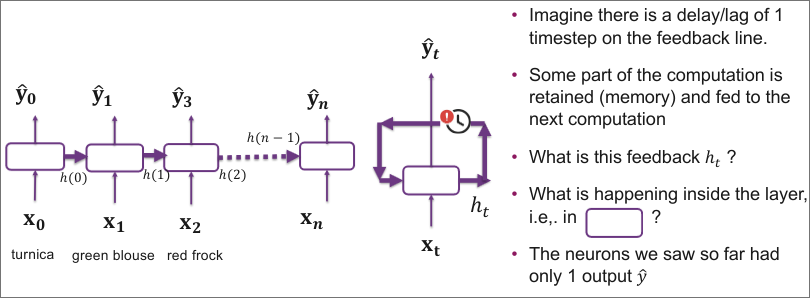
\includegraphics[scale=0.4]{2023_03_20_02_11_18.png}
\subsubsection{Memory Cell}
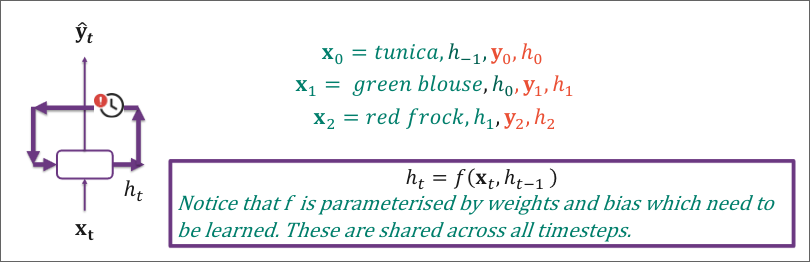
\includegraphics[scale=0.4]{2023_03_20_02_11_30.png}
\subsubsection{simpleRNNCell (keras)}
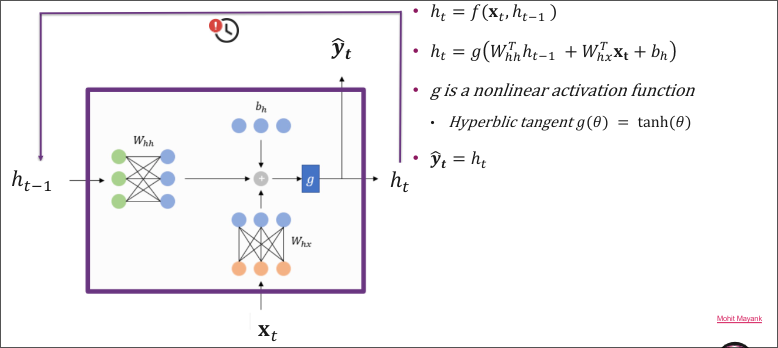
\includegraphics[scale=0.4]{2023_03_20_02_13_13.png}
\subsubsection{Conputations across time/Forward Propagation}
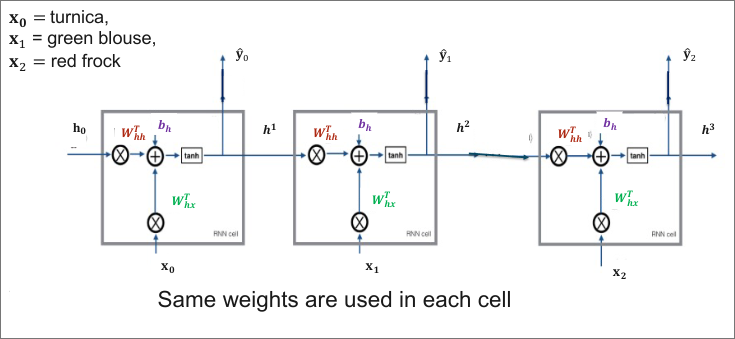
\includegraphics[scale=0.4]{2023_03_20_02_13_34.png}
\subsubsection{How to train RNN?}
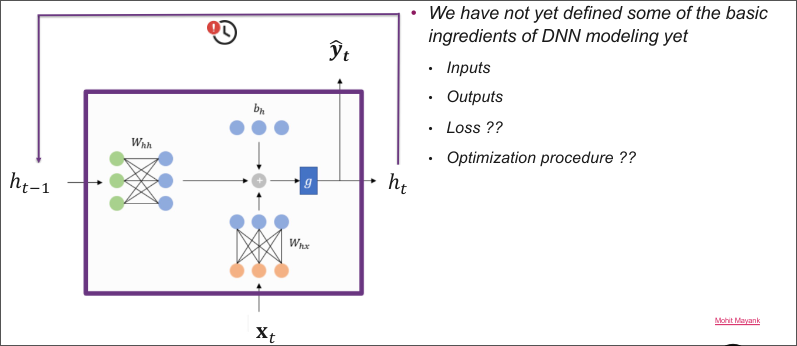
\includegraphics[scale=0.4]{2023_03_20_02_26_37.png}
\subsubsection{Loss across time steps}
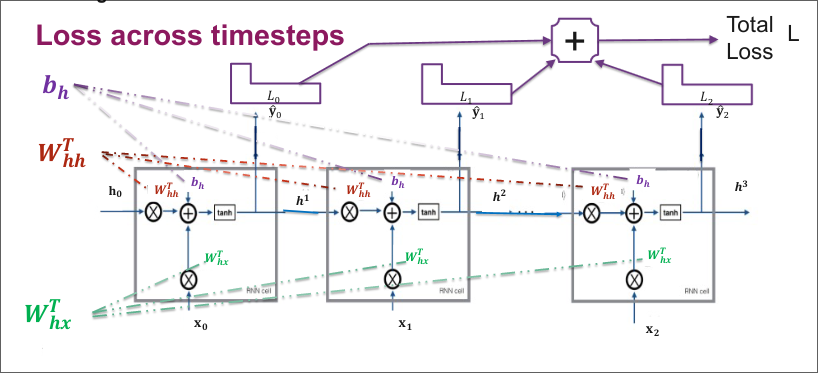
\includegraphics[scale=0.4]{2023_03_20_02_40_41.png}
\subsubsection{Backpropagation through Time}
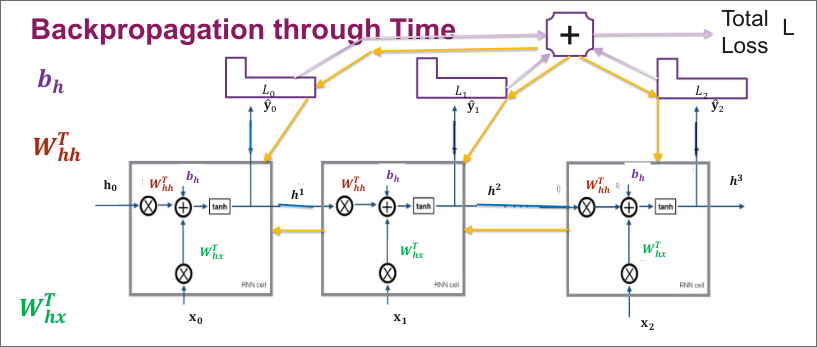
\includegraphics[scale=0.4]{2023_03_20_02_40_58.png}


\subsection{Deep RNN}
\textcolor{teal}{This is the chaining of multiple RNN}\newline
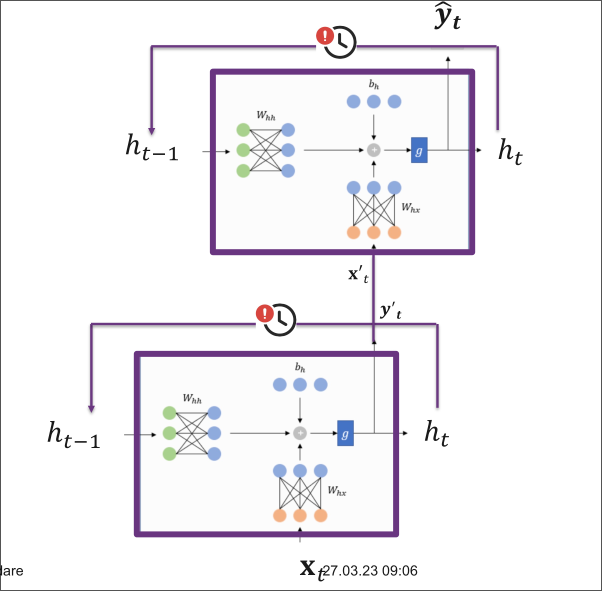
\includegraphics[scale=0.4]{2023_03_27_02_11_52.png}
\subsubsection{Unroll}
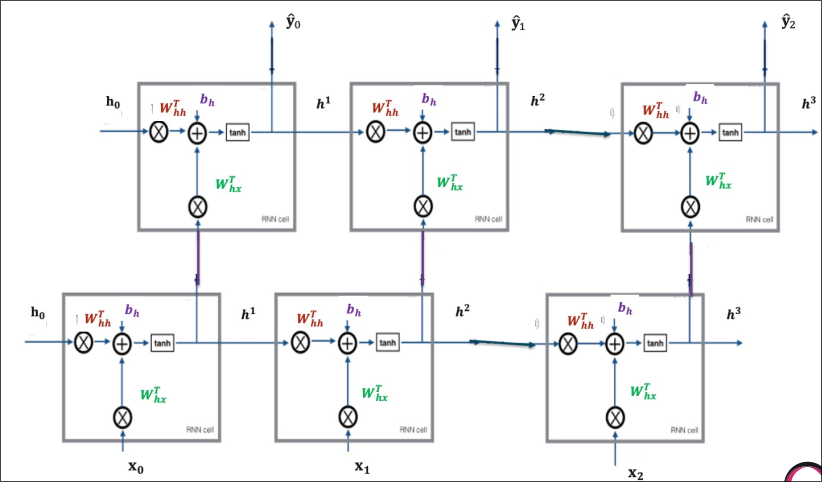
\includegraphics[scale=0.4]{2023_03_27_02_12_48.png}
\subsubsection{Bi-Directional RNN}
\textcolor{teal}{This is an RNN that can propagate from both sides, meaning you can figure out what is necessary in the middle.}\newline
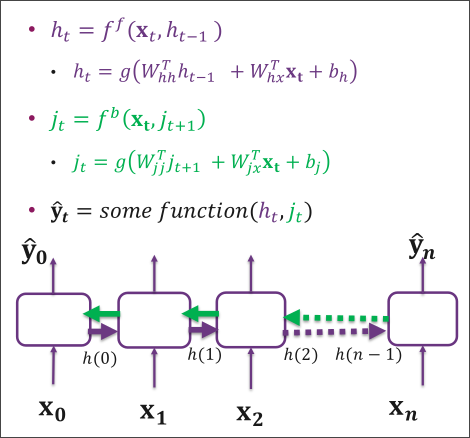
\includegraphics[scale=0.4]{2023_03_27_02_13_11.png}\newline
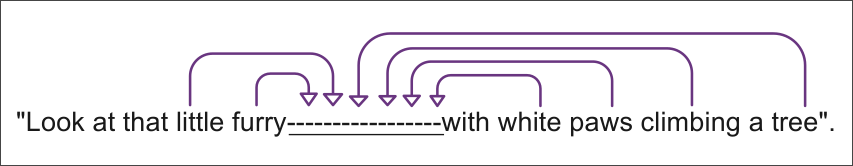
\includegraphics[scale=0.4]{2023_03_27_02_13_44.png}
\subsubsection{Backpropagation through time BPTT}
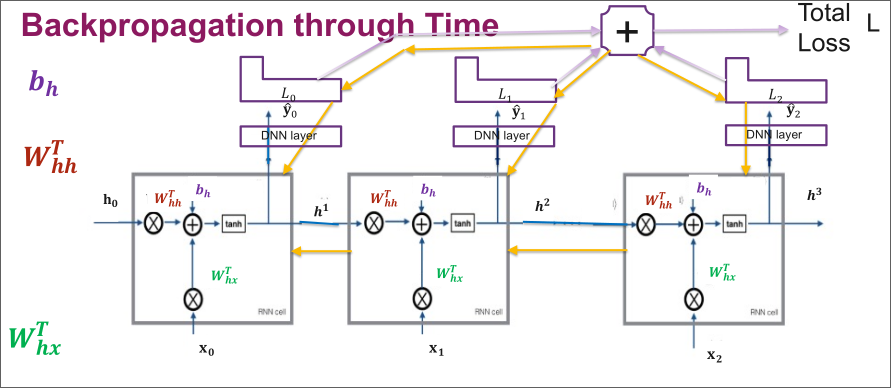
\includegraphics[scale=0.4]{2023_03_27_02_14_31.png}
\subsubsection{Vanishing gradient of simple/vanilla RNNs}
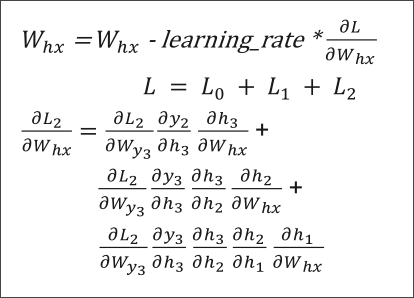
\includegraphics[scale=0.4]{2023_03_27_02_15_07.png}
\subsubsection{Solutions to the problem of backpropagation}
\textcolor{teal}{It gets harder and harder to pass the loss back to time... so wee need a soltion:}\newline
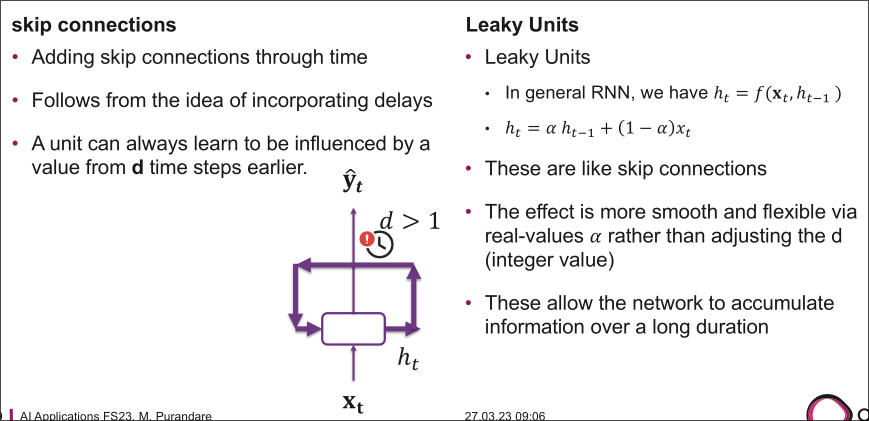
\includegraphics[scale=0.4]{2023_03_27_02_17_50.png}\newline
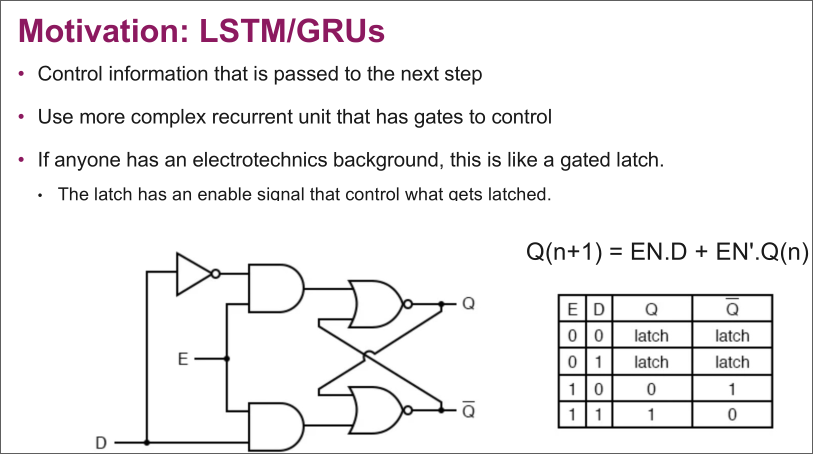
\includegraphics[scale=0.4]{2023_03_27_02_18_59.png}
\subsubsection{Efficient Solution: Gated RNNs}
\begin{itemize}
\item \textcolor{black}{Include long and short-term memory LSTM, and gated recurrent unit GRU models}
\item \textcolor{black}{Generalized versions of leaky units}\newline
  Connection weights e.g. \(\alpha\) may change at each time step
\item \textcolor{black}{Addition to leaky units}\newline
  Once the information is used, neural network can forget the old state 
\item \textcolor{black}{Hot research field..}
\end{itemize} 
\subsubsection{LSTM}
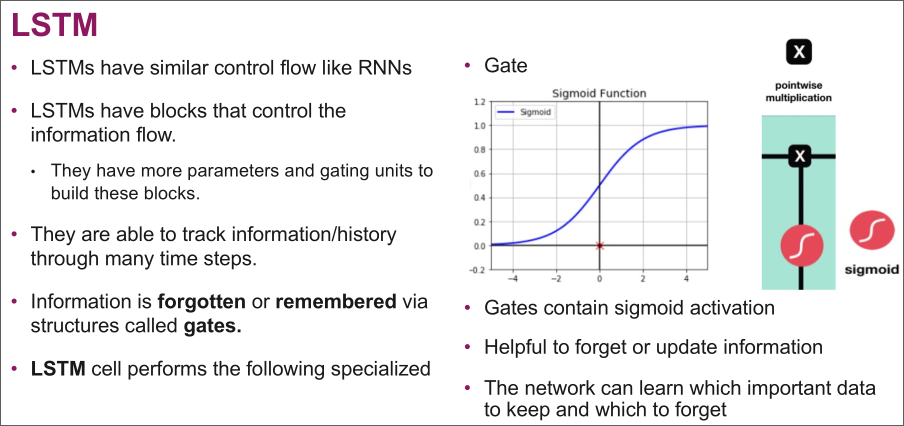
\includegraphics[scale=0.4]{2023_03_27_02_21_21.png}\newline
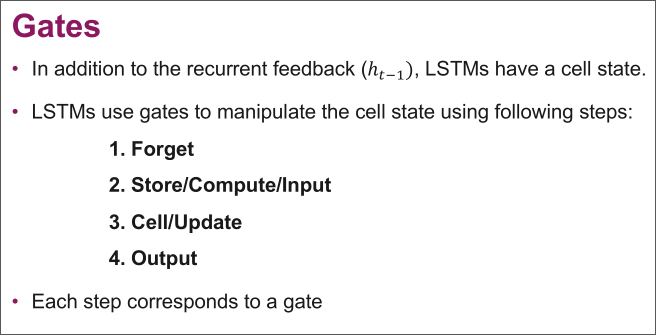
\includegraphics[scale=0.4]{2023_03_27_02_21_38.png}\newline
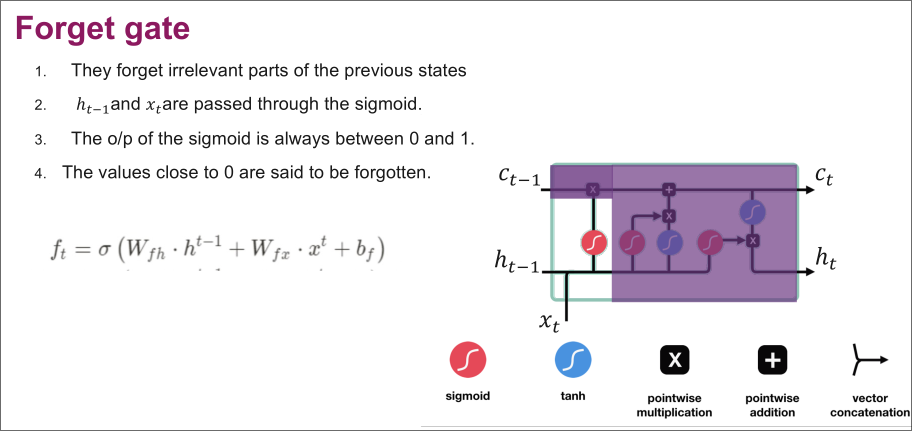
\includegraphics[scale=0.4]{2023_03_27_02_21_56.png}\newline
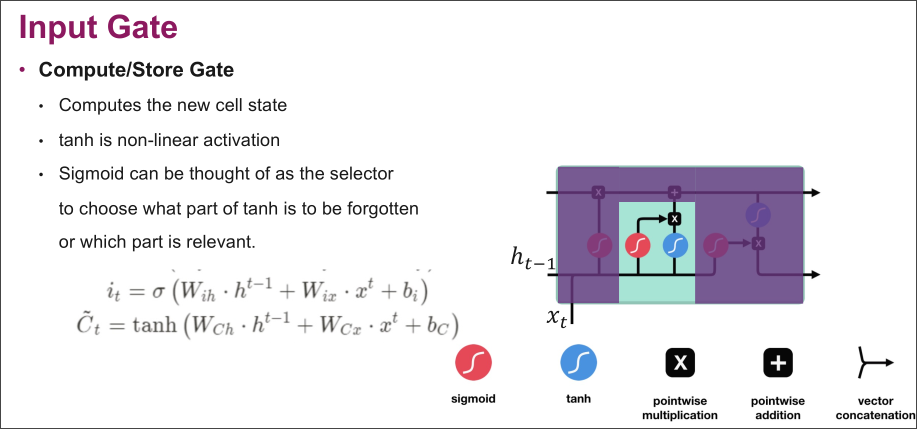
\includegraphics[scale=0.4]{2023_03_27_02_22_10.png}\newline
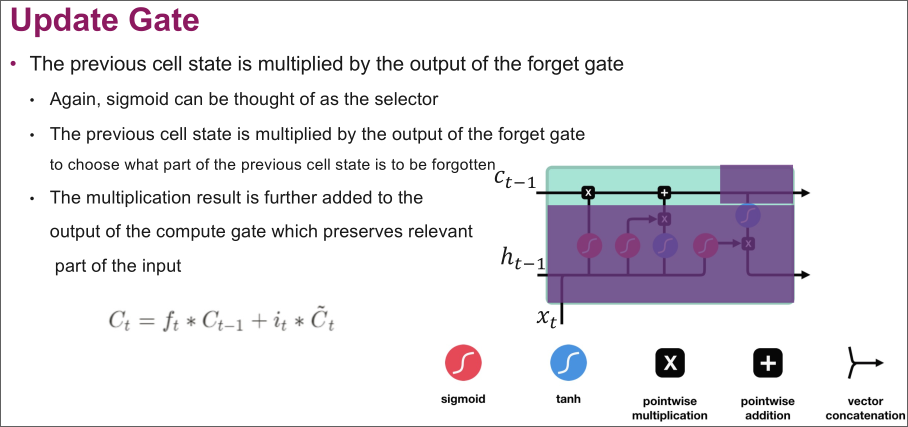
\includegraphics[scale=0.4]{2023_03_27_02_22_27.png}\newline
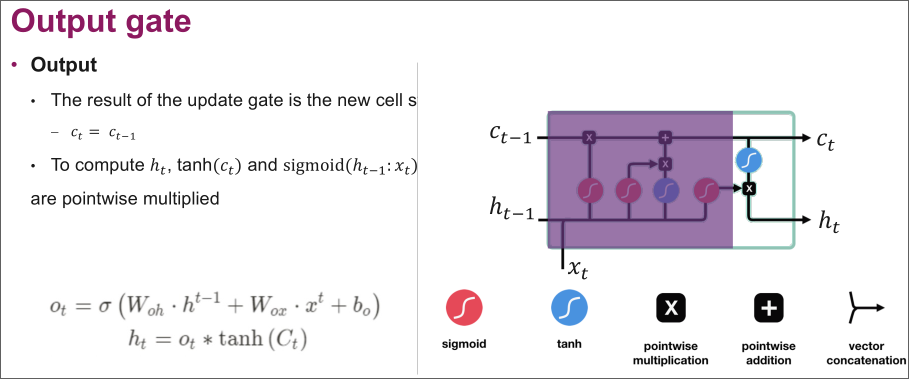
\includegraphics[scale=0.4]{2023_03_27_02_22_46.png}\newline
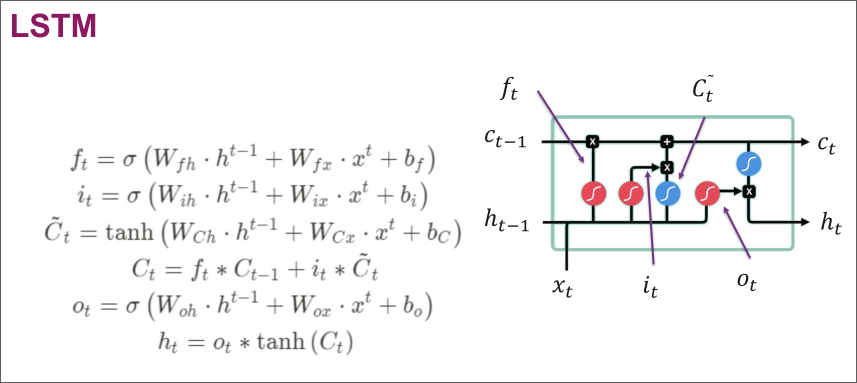
\includegraphics[scale=0.4]{2023_03_27_02_23_01.png}\newline
\includegraphics[scale=0.4]{2023_03_27_02_37_06.png}\newline
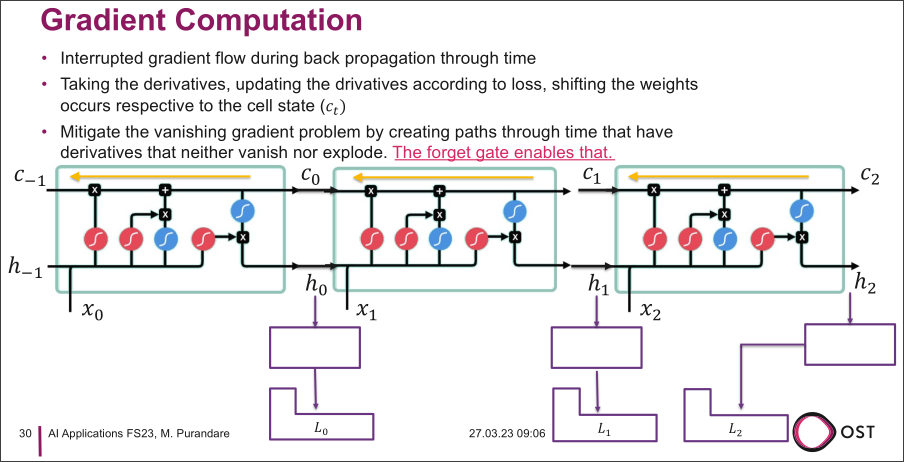
\includegraphics[scale=0.4]{2023_03_27_02_37_42.png}

\subsubsection{Gated Recurrent Units GRU}
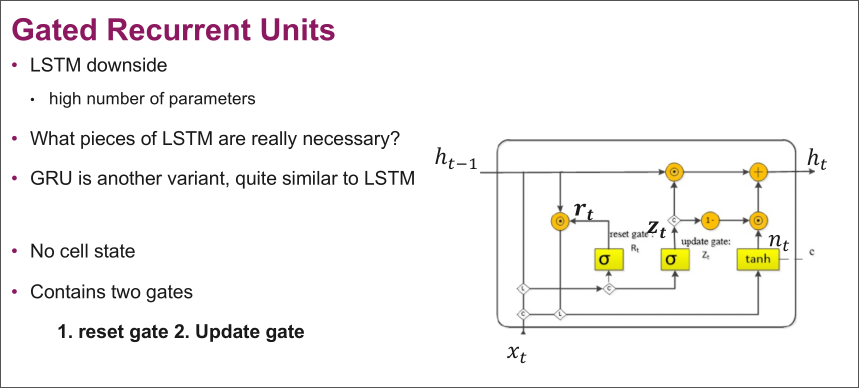
\includegraphics[scale=0.4]{2023_03_27_02_38_16.png}\newline
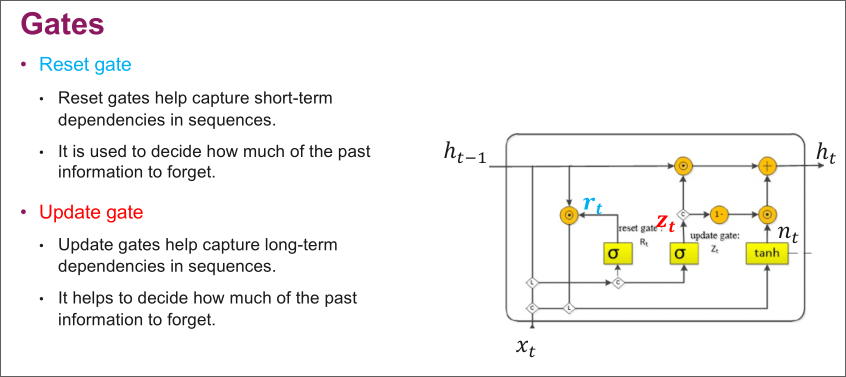
\includegraphics[scale=0.4]{2023_03_27_02_38_29.png}\newline
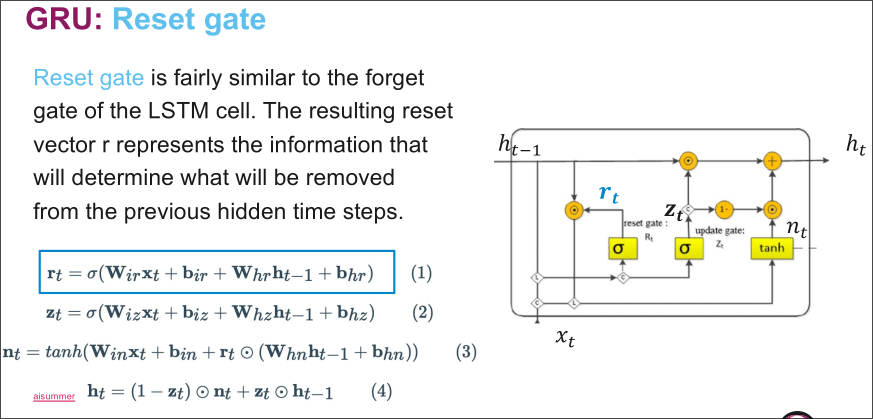
\includegraphics[scale=0.4]{2023_03_27_02_38_47.png}\newline
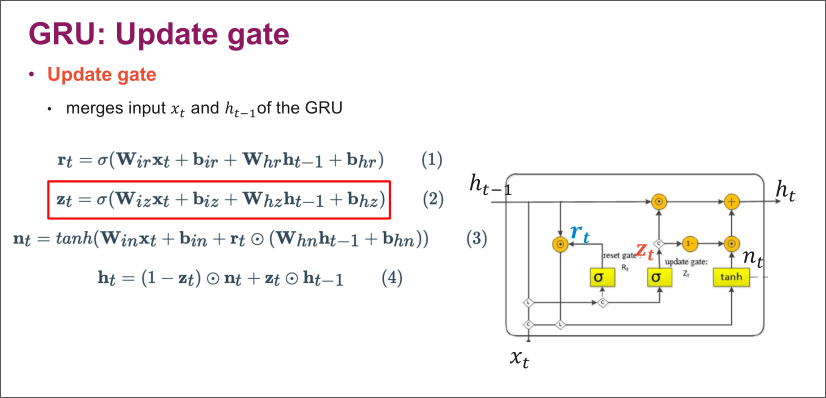
\includegraphics[scale=0.4]{2023_03_27_02_39_00.png}\newline
\includegraphics[scale=0.4]{2023_03_27_02_39_11.png}\newline
\includegraphics[scale=0.4]{2023_03_27_02_39_23.png}\newline

\subsubsection{LSTM vs GRU}
\begin{itemize}
\item \textcolor{black}{LSTM is a bigger and more expensive model}
\item \textcolor{black}{GRU is faster and compacter}
\item \textcolor{black}{LSTM should only be used if you have a reason for it}
\item \textcolor{black}{LSTM should remember longer sequences than GRU}
\item A GRU has one less gate than LSTM. Precisely, just a reset and update gates instead of the forget, input and output gate of LSTM.
\end{itemize} 


\subsection{Seq2seq}
This is the split of an RNN cell into an encoder and a decoder part.\newline
The encoder gives the sequence to the decoder as well as the \emph{context}, which are the "important" parts of the input.\newline
This results in less "memorizing" of old state, while not giving up on accuracy.\newline
\includegraphics[scale=0.4]{2023_04_03_01_52_46.png}

\subsubsection{Encoder}
\includegraphics[scale=0.4]{2023_04_03_02_07_09.png}

\subsubsection{Decoder}
\includegraphics[scale=0.4]{2023_04_03_02_07_36.png}

\subsubsection{Problems}
\includegraphics[scale=0.4]{2023_04_03_02_22_32.png}\newline
\textcolor{teal}{The biggest issue with this is the fact that this is not \emph{parallelizeable}, it must perform each seuence in a serial manner}

\subsection{Transformers}
\textcolor{red}{This is the solution to the seq2seq problem. Unlike the last model this is parallizeable. \newline
It is what powers ChatGPT, and it is what makes the new generation of AI so powerful}\newline
\includegraphics[scale=0.4]{2023_04_03_02_25_34.png}\newline
\textcolor{red}{Note, \emph{Transformers do NOT use any recurrence}}

\subsubsection{Attention}
Transformers only really care about the concept of "attention", which is comprised of \emph{Query, key, value}.\newline
\includegraphics[scale=0.4]{2023_04_03_02_36_51.png}\newline
\includegraphics[scale=0.4]{2023_04_03_02_37_04.png}\newline
Essentially you check how similar the key is to the query.\newline
\includegraphics[scale=0.4]{2023_04_03_02_38_12.png}\newline
\includegraphics[scale=0.4]{2023_04_03_02_38_33.png}\newline
Lastly you multiply the result with the value, which results in the output.\newline
\includegraphics[scale=0.4]{2023_04_03_02_39_02.png}\newline
Decoder and Encoder example with Attention instead of reccurence\newline
\includegraphics[scale=0.4]{2023_04_03_02_44_18.png}

\end{document}
